\documentclass{article}

\usepackage[utf8]{inputenc}

\usepackage{geometry}
\geometry{a4paper}

\usepackage{titling}

\usepackage{tikz}
\tikzstyle{every node}=[circle, draw, fill=black!50, inner sep=0pt, minimum width=4pt]

\usepackage{amsmath}
\usepackage{amssymb}
\usepackage{amsfonts}


\begin{document}

\title{Examen final matematica discreta 2016}
\date {}
\maketitle

\begin{enumerate}
\item Sea $G$ un grafo con $n > 1$ vertices y $m$ aristas:
\begin{enumerate}
\item Probar que si $m > \frac{(n-1)(n-2)}{2}$, entonces $G$ es conexo.
\item Si $m = \frac{(n-1)(n-2)}{2}$, ¿es $G$ necesariamente conexo?
\end{enumerate}
\item Sea $G$ un grafo con grado minimo $\delta \geq 2$
\begin{enumerate}
\item Probar que $G$ contiene un camino de longitud al menos $\delta$. [Indicacion: considerad
el camino en $G$ de longitud maxima]
\item Probar que $G$ contiene un ciclo de longitud al menos $\delta + 1$
\end{enumerate}
\item \begin{enumerate}
\item Sea $G$ un grafo bipartido planario. Probar que $\delta(G) \leq 3$.
\item Sea $G$ un grafo planario con $n$ vertices donde todos los ciclos tienen al menos
longitud $g$, con $g \geq 3$. Probar que el numero de aristas $m$ satisface
\[
m \leq \frac{g}{g-2}n - \frac{2g}{g-2}
\]
\end{enumerate}
\item \begin{enumerate}
\item Sea $G = (V, A)$ un grafo aciclico (un bosque) con $n$ vertices y $c$ componentes conexas.
Probar que
\[
2c + \sum_{x \in V}(g(x) - 2) = 0
\]
\item Sea $F$ el arbol infinito con un conjunto de vertices $V$ donde todos los vertices tienen grado
exactamente 4. Para cualquier subconjunto finito $A$ de $V$ definimos el borde de $A$ como
\[
\partial A = \left\{ v \in A \mid v \text{ es adyacente a al menos un vertice de } V\setminus A \right\}
\]
Probar que todo subconjunto finito y no vacio $A \subset V$ cumple
\[
\frac{\lvert \partial A \rvert}{\lvert A \rvert} > \frac{2}{3}
\]
[Indicacion: Pensad $A$ como un grafo aciclico y completad $\lvert A \rvert$ distinguiendo los grados
de los vertices]
\item Probar que $F$ tiene la siguiente propiedad:
\[
\inf_{\substack{\emptyset \neq A \subset V \\ A \text{ finito}}}
\left\{ \frac{\lvert \partial A \rvert}{\lvert A \rvert} \right\} = \frac{2}{3}
\]
[Indicacion: Considerad las ``bolas'' $B(n) = \{v \in V \mid d(v_0,v) \leq n\}$, donde $v_0$ es un
vertice fijo cualquiera]
\end{enumerate}
\end{enumerate}

\newpage
%==========================
\title{Solucion}
\date{}
\maketitle

\begin{enumerate}
\item \begin{enumerate}
\item Razonamos por reduccion al absurdo, suponemos que $G$ no es conexo, entonces existe
$G_1$ una componente conexa y $G_2 = G \setminus G_1$ que contienen $p$ y $n-p$ vertices
respectivamente. Sean $a_1$ y $a_2$ el numero de aristas $G_1$ y de $G_2$,
entonces se tiene
\[
m = a_1 + a_2 \leq \frac{p(p-1)}{2} + \frac{(n-p)(n-p-1)}{2} = \frac{n^2 -2np -n +2p^2}{2}
\]
Por otro lado
\[
 \frac{n^2 -2np -n +2p^2}{2} \geq m > \frac{(n-1)(n-2)}{2} = \frac{n^2-3n+2}{2} \iff
 \]
 \[
 \iff
 -2np +2p^2 > -2n + 2
 \iff
 p^2 > n(p-1) + 1
 \iff p > n
\]
Lo cual es una contradiccion, ya que $G_1$ no puede contener mas de $n$ vertices
\item No, el grafo

\begin{center}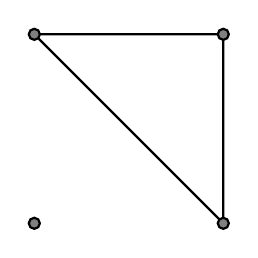
\begin{tikzpicture}[thick,scale=0.8]
\def \n {1.5}
\draw
(-\n,\n) node{} -- (\n,\n)
(\n,\n) node{} -- (\n,-\n) node{}
(-\n,\n) -- (\n,-\n)
(-\n,-\n) node{};
\end{tikzpicture}\end{center}
tiene 4 vertices y $\frac{(4-1)(4-2)}{2}=3$ aristas, pero no es conexo.
\end{enumerate}


%=======================


\item \begin{enumerate}
\item Sea $C = v_1, \cdots, v_p$ el camino de longitud maxima en $G$. Razonamos ahora por reduccion
al absurdo. Suponemos que $p < \delta$, pero $\delta(v_1) \geq \delta$ y por lo tanto, $v_1$ esta
conectado a un vertice $u$ fuera de $C$ y el camino $u, v_1, \cdots, v_p$ es mas largo que
$C$ lo cual es una contradiccion. Entonces, nuestra hipotesis es falsa, es decir $p \geq \delta$

\item De nuevo, sea $C = v_1, \cdots, v_p$ el camino de longitud maxima en $G$, y, por el apartado a, $p \geq \delta$ y $v_1$ es adyacente a, al menos, $\delta$ vertices de este camino (no puede
estar unido a ninguno fuera, ya que entonces existiria un camino mas largo). Aplicando ahora el
principio del palomar, sabemos que $\exists q$ tal que $v_1 \sim v_q$ y $\delta \leq q \leq p$, y por lo
tanto, el ciclo $v_1, \cdots, v_q, v_1$ tiene longitud $q+1 \geq \delta + 1$ 
\end{enumerate}


%=====================


\item \begin {enumerate}
\item Como $G$ es planario, cumple la relacion de $c + n = m + 2$, donde $c$ es el numero de caras,
$n$ el numero de vertices y $m$ el numero de aristas. Ahora, tenemos que 
\[
4c \leq \sum_{i = 1}^{c} f_i \leq 2m
\]
Donde $f_i$ son el numero de aristas de la cara $i$. Esta relacion se tiene debido a que cada cara
esta limitada por al menos 4 aristas (ya que no hay ciclos impares y no puede haber una cara de borde
3), y una arista es borde de como mucho 2 caras. Por lo tanto:
\[
4c \leq 2m \iff 4(m + 2 - n) \leq 2m \iff m \leq 2n - 4
\]
Suponemos ahora que $\delta(G) \geq 4$ y por lo tanto:
\[
\sum_{x \in G} g(x) = 2m \geq 4n 
\]
Pero aplicando el resultado anterior, obtenemos:
\[
2n -4 \geq m \geq 2n
\]
Como es falso, nuestra hipotesis de partida es falsa, es decir $\delta(G) < 4 \iff \delta(G) \leq 3$

\item De nuevo, como $G$ es planario, cumple $c + n = m +2$ donde $c$ es el numero de caras
$n$ el numero de vertices y $m$ el numero de aristas. Tenemos ahora que:
\[
gc \leq \sum_{i=1}^{c} f_i \leq 2m
\]
Donde $f_i$ son el numero de aristas de la cara $i$.  Esta relacion se tiene debido a que cada cada cara
esta limitada por al menos $g$ aristas (si no existiria un ciclo de longitud menor a $g$) y cada arista
pertenece como mucho a dos caras. Aplicando el resultado anterior, se tiene
\[
g(m+2-n) \leq 2m \iff m(g-2) \leq g(n-2) \iff m \leq \frac{g}{g-2}n + \frac{2g}{g-2}
\]
\end{enumerate}


%================


\item \begin{enumerate}
\item Llamando $C_1, \cdots, C_c$ a las componentes conexas, podemos reescribir la expresion
del enunciado como
\[
2c + \sum_{i=0}^{c} \left( \sum_{x \in C_i} g(x) - 2 \right) =
2c + \sum_{i=0}^{c} \left( 2 m_i - 2 \lvert C_i \rvert \right)
\]
Donde $m_i$ es el numero de aristas de $C_i$. Pero como $C_i$ es un arbol, tenemos que
$m_i = \lvert C_i \rvert - 1$ y sustituyendo:
\[
2c + \sum_{i=0}^{c} \left(2(\lvert C_i \rvert - 1) - 2 \lvert C_i \rvert \right) = 
2c + \sum_{i=0}^{c} -2 = 2c -2c = 0
\]

 \item Sean $C_1, \cdots, C_n$ las componentes conexas de $A$, como $F$ es un arbol, $C_i$
 tambien es un arbol, y por lo tanto el numero de aristas que tiene es $\lvert C_i \rvert -1$, pero cada
 vertice tiene grado 4, por lo tanto:
 \[
 4 \lvert C_i \rvert = g(C_i) + 2(\lvert C_i \rvert -1)
 \]
 Donde $g(C_i)$ es el numero de aristtas que unen un vertice de $C_i$ con uno del exterior. Entonces
 $g(C_i) = 2 \lvert C_i \rvert + 2$, pero, como cada vertice de $C_i$ tiene como mucho 3 aristas que le
 conectan con el exterior (el caso $\lvert C_i \rvert = 1$ lo contemplaremos mas adelante), entonces:
 \[
 \lvert \partial C_i \rvert \geq \frac{2}{3}\lvert C_i \rvert + \frac{2}{3}
 \iff
\lvert \partial C_i \rvert >\frac{2}{3}\lvert C_i \rvert
 \]
 En el caso $\lvert C_i \rvert = 1$, tenemos $\lvert \partial C_i \rvert = $ y por lo tanto:
 $\lvert \partial C_i \rvert = 1 > \frac{2}{3}\lvert C_i \rvert = \frac{2}{3}$. Ahora tenemos que:
 \[
 \frac{\lvert \partial A \rvert}{\lvert A \rvert} =
 \frac{\lvert \partial C_1 \rvert + \cdots + \lvert \partial C_n \rvert}
 {\lvert C_1 \rvert + \cdots + \lvert C_n \rvert} >
 \frac{\frac{2}{3}\lvert C_1 \rvert + \cdots + \frac{2}{3}\lvert C_n \rvert}
 {\lvert C_1 \rvert + \cdots + \lvert C_n \rvert } =
 \frac{\frac{2}{3} \left( \lvert C_1 \rvert + \cdots + \lvert C_n \rvert \right)}
 {\lvert C_1 \rvert + \cdots + \lvert C_n \rvert } = \frac{2}{3}
 \]
 
 \item Consideramos las bolas $B(n)$, ya definidas (tomando como centro un vertice aleatorio).
 Primero, consideramos $B(1)$:
 
\begin{center}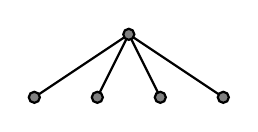
\begin{tikzpicture}[thick,scale=0.8]
\def \n {1}
\def \m {1}
\draw
(0,0) node {}
\foreach \x in {1,2,...,4} {
	(0,0)  -- (\m*\x-\m*2.5,-\n) node{}
 };
\end{tikzpicture}\end{center}
Como se puede observar, $\lvert B(1) \rvert = 5$ y $\lvert \partial B(1) \rvert = 4$. Consideramos $B(2)$:
\begin{center}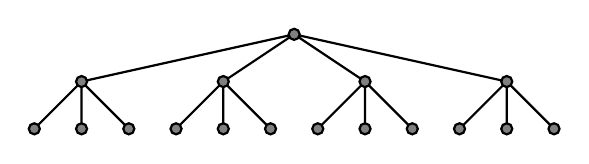
\begin{tikzpicture}[thick,scale=0.8]
\def \n {.75}
\def \m {.75}
\draw
(0,0) node {}
\foreach \x in {1,2,...,4} {
	(0,0)  -- (3*\m*\x-7.5*\m,-\n) node{}
	\foreach \y in {1,2,3} {
		(3*\m*\x-7.5*\m,-\n) -- (3*\m*\x + \y*\m - 9.5*\m, -2*\n) node{}
	}
 };
\end{tikzpicture}\end{center}
Donde $\lvert B(2) \rvert = 17$ y $\lvert \partial B(2) \rvert = 12$. Mas en general, en $B(n)$:
\tikzstyle{white}=[draw=none,fill=none]
\begin{center}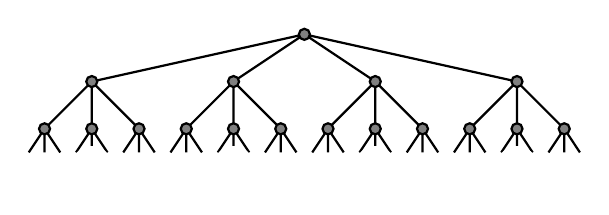
\begin{tikzpicture}[thick,scale=0.8]
\def \n {.75}
\def \m {.75}
\draw
(0,0) node {}
\foreach \x in {1,2,...,4} {
	(0,0)  -- (3*\m*\x-7.5*\m,-\n) node{}
	\foreach \y in {1,2,3} {
		(3*\m*\x-7.5*\m,-\n) -- (3*\m*\x + \y*\m - 9.5*\m, -2*\n) node{}
		\foreach \z in {1,2,3} {
			(3*\m*\x + \y*\m - 9.5*\m, -2*\n) -- (3*\m*\x + \y*\m + \z*\m*0.333 -10.1666*\m, -2.5*\n)
		}
	}
	(3*\m*\x-7.5*\m,-2.8*\n) node[white]{$\cdots$}
 };
\end{tikzpicture}\end{center}
Se tiene que $\lvert B(n) \rvert = 1 + 4(3^0 + \cdots + 3^{n-1})$ y
$\lvert \partial B(n) \rvert = 4\times3^{n-1}$, ya que a cada nivel se añaden tres veces los vertices del
nivel anterior. Ahora hacemos:
\[
\lim_{n \to \infty} \frac{\lvert \partial B(n) \rvert}{\lvert B(n) \rvert} =
\lim_{n \to \infty} \frac{4\times3^{n-1}}{1 + 4(3^0 + \cdots + 3^{n+1}}
\]
Pero $(3^0 + 3^1 + \cdots + 3^{n-1}) = \frac{3^n-1}{2}$, entonces 
\[
\lim_{n \to \infty} \frac{4\times3^{n-1}}{1 + 4 \frac{3^n - 1}{2}} = 
\lim_{n \to \infty} \frac{4\times3^{n-1}}{2\times 3^n - 1} = 
\lim_{n \to \infty} \frac{2}{3 - \frac{1}{3^{n-1}}} = \frac{2}{3}
\]
Y por lo tanto
\[
\inf_{\substack{\emptyset \neq A \subset V \\ A \text{ finito}}}
\left\{ \frac{\lvert \partial A \rvert}{\lvert A \rvert} \right\} \leq \frac{2}{3}
\]
Pero, por el resultado del apartado b, tenemos que:
\[
\inf_{\substack{\emptyset \neq A \subset V \\ A \text{ finito}}}
\left\{ \frac{\lvert \partial A \rvert}{\lvert A \rvert} \right\} \geq \frac{2}{3}
\]
De donde deducimos que
\[
\inf_{\substack{\emptyset \neq A \subset V \\ A \text{ finito}}}
\left\{ \frac{\lvert \partial A \rvert}{\lvert A \rvert} \right\} = \frac{2}{3}
\]
\end{enumerate}
\end{enumerate}
\end{document}
